\chapter{Perancangan}
\label{chap:design}

Pada bab ini akan dipaparkan berbagai macam rancangan dari perkakas \cl\xspace yang dibuat, seperti diagram-diagram terkait, masukan serta keluaran perangkat lunak, serta detail mengenai fungsi-fungsi yang ada di dalam perkakas tersebut.

\section{Rancangan Alur Kerja Perkakas}
\label{sec:design-flow}

Bagian ini akan membahas mengenai alur kerja perkakas yang dibuat, dalam bentuk \textit{activity diagram} serta \textit{sequence diagram} dari fitur-fitur perkakas. Perkakas memiliki empat buah fitur, yaitu:

\begin{itemize}
	\item menampilkan bantuan penggunaan,
	\item mencari lokasi menggunakan kata kunci pencarian (\verb|searchplace|),
	\item mencari rute dengan angkot menggunakan \latlon\xspace lokasi (\verb|findroute|), dan
	\item mencari rute dengan angkot menggunakan kata kunci pencarian lokasi (\verb|direct|).
\end{itemize}

\noindent
Tiap-tiap fitur akan memiliki satu dari setiap tipe diagram. Kedua tipe diagram diikutkan untuk menggambarkan dengan lebih jelas langkah-langkah kerja perkakas, dengan \textit{activity diagram} menggambarkan \textit{apa saja} aktivitas yang dilakukan oleh tiap-tiap aktor dalam setiap proses kerja perkakas, dan \textit{sequence diagram} menggambarkan \textit{kapan} aktivitas-aktivitas tersebut dilakukan oleh tiap-tiap aktor. Adapun penjelasan dari bagaimana fitur-fitur ini akan diimplementasikan adalah sebagai berikut.

\subsection{Mencari lokasi menggunakan kata kunci pencarian}
\label{sec:design-flow-searchplace}

Alur kerja untuk fitur pencarian lokasi menggunakan kata kunci pencarian adalah sebagai berikut.

\begin{figure}[h]
    \centering
    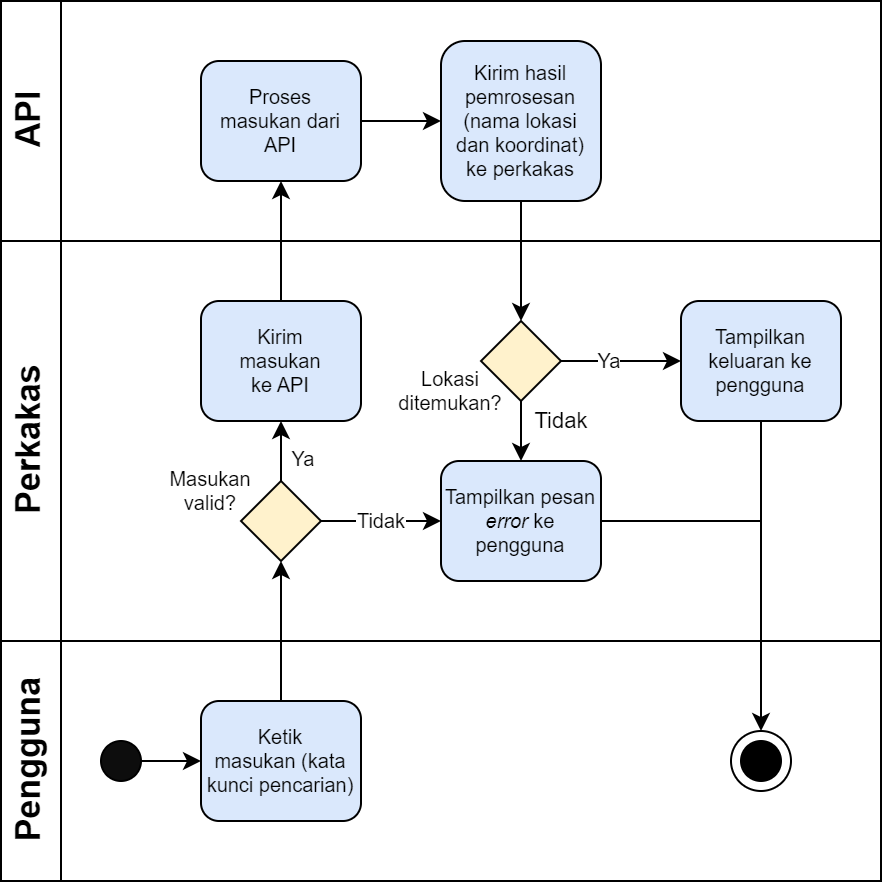
\includegraphics[width=0.55\linewidth]{diagrams-activity-searchplace}
    \caption[\textit{Activity diagram} fitur pencarian lokasi menggunakan kata kunci lokasi]{\textit{Activity diagram} dari fitur pencarian lokasi menggunakan kata kunci pencarian.}
    \label{fig:diagrams-activity-searchplace}
\end{figure}

\begin{figure}[h]
    \centering
    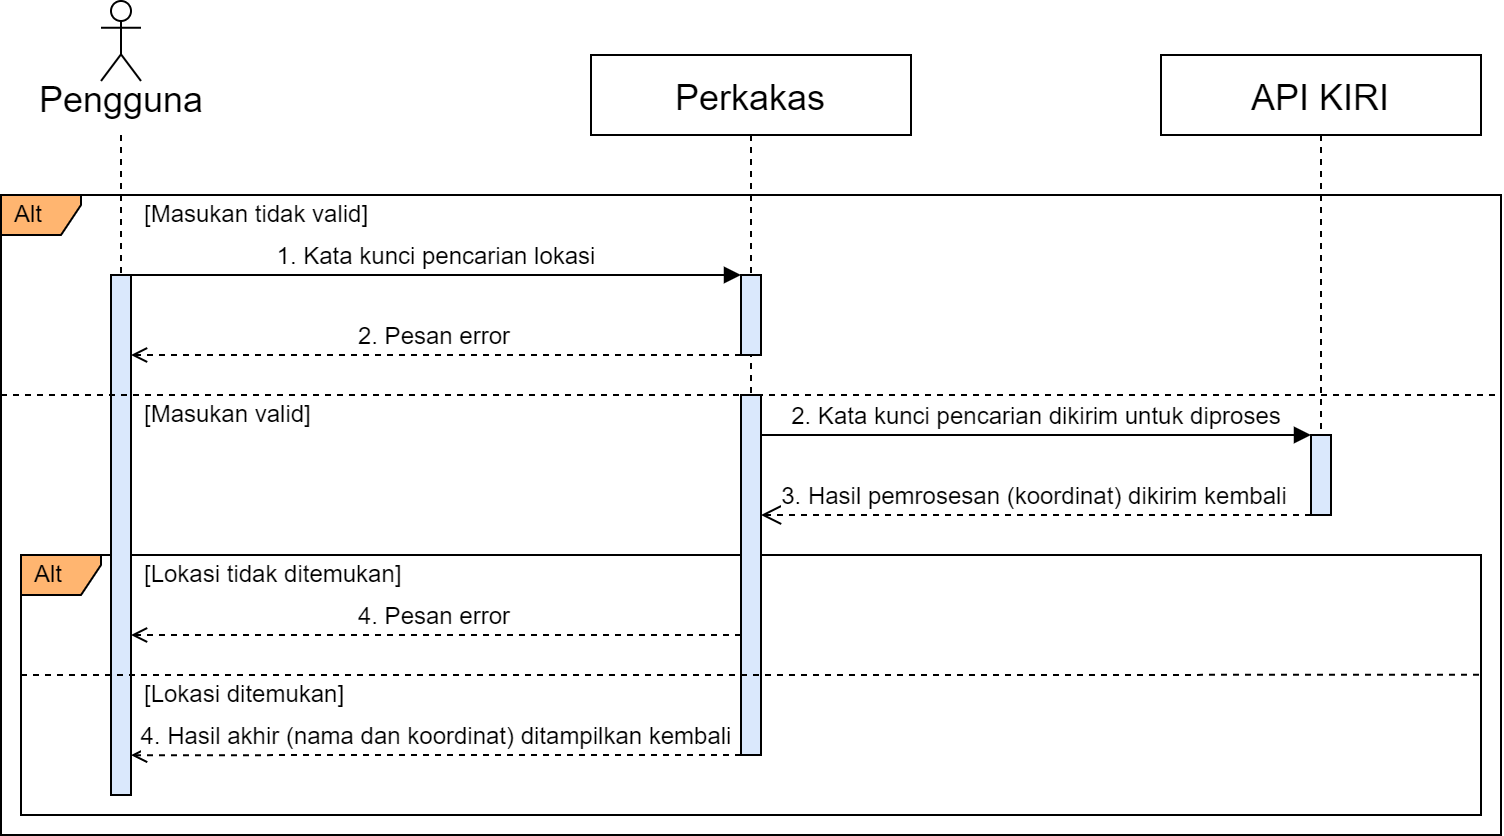
\includegraphics[width=0.8\linewidth]{diagrams-sequence-searchplace}
    \caption[\textit{Sequence diagram} fitur pencarian lokasi menggunakan kata kunci lokasi]{\textit{Sequence diagram} dari fitur pencarian lokasi menggunakan kata kunci pencarian.}
    \label{fig:diagrams-sequence-searchplace}
\end{figure}

\begin{enumerate}
	\item Perkakas akan meminta masukan dari pengguna berupa kata kunci dari lokasi yang ingin dicari.
	\item Masukan akan dicek oleh perkakas validitasnya. Dalam kasus ini, masukan hanya akan dianggap tidak valid apabila pengguna tidak memasukkan apa pun sebagai masukan perkakas (masukan kosong).
	\item Jika kata kunci masukan:

	\begin{itemize}
		\item tidak valid, maka perkakas akan mengeluarkan pesan \textit{error} dan keluar.
		\item dianggap valid, kata kunci tersebut akan dikirim ke API KIRI untuk diproses lebih lanjut.
	\end{itemize}
	
	\item Setelah selesai diproses, keluaran dari API akan dikembalikan ke perkakas.
	\item Perkakas akan mengecek keluaran yang diterimanya. Apabila lokasi:
	
	\begin{itemize}
		\item ditemukan, maka nama dan koordinat \latlon\xspace lokasi akan ditampilkan ke pengguna sebagai keluaran akhir.
		\item tidak ditemukan, maka perkakas akan mengeluarkan pesan \textit{error} dan keluar.
	\end{itemize}
	
	Perlu ditekankan bahwa perkakas tidak peduli apakah lokasi yang ditemukan benar (sesuai dengan yang diinginkan pengguna) atau tidak.
	
\end{enumerate}
\noindent
Dengan alur tersebut, maka dapat dibuat sepasang diagram untuk fitur ini, di mana \textit{activity diagram}-nya dapat dilihat di Gambar \ref{fig:diagrams-activity-searchplace}, dan \textit{sequence diagram}-nya dapat dilihat di Gambar \ref{fig:diagrams-sequence-searchplace}.
\newpage\vspace*{-3em} % prevent widow
\subsection{Mencari rute dengan angkot menggunakan \latlon\xspace lokasi}
\label{sec:design-flow-findroute}

Alur kerja untuk fitur pencarian rute angkot menggunakan koordinat \latlon\xspace lokasi awal dan akhir adalah sebagai berikut.

\begin{figure}[h]
    \centering
    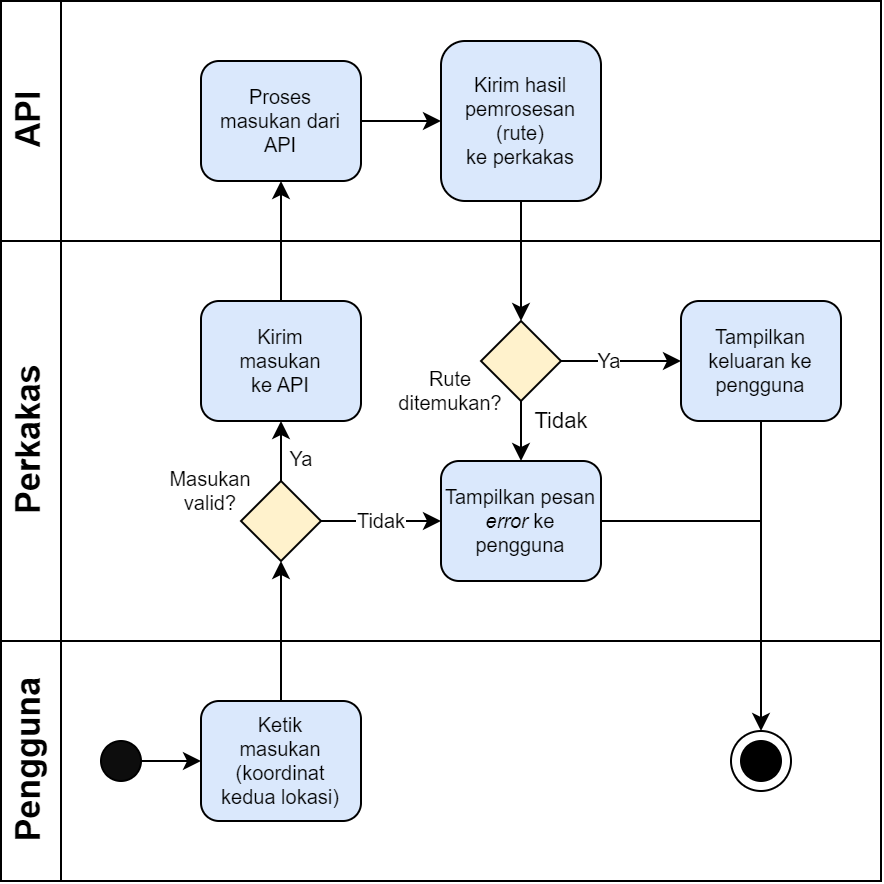
\includegraphics[width=0.55\linewidth]{diagrams-activity-findroute}
    \caption[\textit{Activity diagram} fitur pencarian rute angkot menggunakan koordinat lokasi]{\textit{Activity diagram} dari fitur pencarian rute angkot menggunakan \latlon\xspace lokasi.}
    \label{fig:diagrams-activity-findroute}
\end{figure}

\begin{figure}[h]
    \centering
    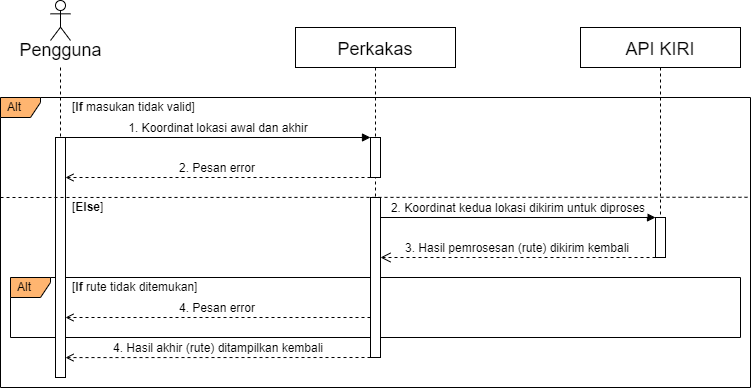
\includegraphics[width=0.8\linewidth]{diagrams-sequence-findroute}
    \caption[\textit{Sequence diagram} fitur pencarian rute angkot menggunakan koordinat lokasi]{\textit{Sequence diagram} dari fitur pencarian rute angkot menggunakan \latlon\xspace lokasi.}
    \label{fig:diagrams-sequence-findroute}
\end{figure}

\begin{enumerate}
	\item Perkakas akan meminta dua buah masukan dari pengguna, berupa koordinat \latlon\xspace dari lokasi awal (mulai) dan lokasi akhir (tujuan).
	\item Masukan akan dicek oleh perkakas validitasnya. Dalam kasus ini, masukan akan dianggap tidak valid apabila ada masukan yang bukan berupa koordinat \latlon .
	\item Jika:
	
	\begin{itemize}
		\item satu atau lebih masukan tidak valid, maka perkakas akan mengeluarkan pesan \textit{error} dan keluar.
		\item kedua masukan dianggap valid, kedua koordinat tersebut akan dikirim ke API KIRI untuk diproses lebih lanjut.
	\end{itemize}
	 
	\item Setelah selesai diproses, keluaran dari API akan dikembalikan ke perkakas.
	\item Perkakas akan mengecek keluaran yang diterimanya. Apabila rute:
	
	\begin{itemize}
		\item berhasil ditemukan (ada setidaknya satu langkah dalam rute), maka rute tersebut akan ditampilkan ke pengguna sebagai keluaran akhir.
		\item tidak berhasil ditemukan, maka perkakas akan mengeluarkan pesan \textit{error} dan keluar.
	\end{itemize}
	
\end{enumerate}
\noindent
Dengan mengikuti alur kerja fitur yang telah dipaparkan, maka dapat dibuat sepasang diagram, yaitu \textit{activity diagram} yang dapat dilihat di Gambar \ref{fig:diagrams-activity-findroute}, dan \textit{sequence diagram} yang dapat dilihat di Gambar \ref{fig:diagrams-sequence-findroute}. 

\subsection{Mencari rute dengan angkot menggunakan kata kunci pencarian lokasi}
\label{sec:design-flow-directroute}


Alur kerja dari fitur pencarian rute angkot menggunakan kata kunci pencarian lokasi adalah sebagai berikut.

\begin{enumerate}
	\item Perkakas akan meminta masukan dari pengguna berupa kata kunci dari lokasi awal dan lokasi akhir yang ingin dicari.
	\item Masukan untuk lokasi awal akan dicek oleh perkakas validitasnya. Dalam kasus ini, masukan hanya akan dianggap tidak valid apabila pengguna tidak memasukkan apa pun (masukan kosong), atau memasukkan koordinat \latlon\xspace sebagai masukan perkakas.
	\item Jika kata kunci masukan:
	
	\begin{itemize}
		\item tidak valid, maka perkakas akan mengeluarkan pesan \textit{error} dan keluar.
		\item dianggap valid, kata kunci tersebut akan dikirim ke API KIRI untuk diproses lebih lanjut.
	\end{itemize}
	 
	\item Setelah selesai diproses, keluaran dari API akan dikembalikan ke perkakas.
	\item Perkakas akan mengecek keluaran yang diterimanya. Apabila lokasi:
	
	\begin{itemize}
		\item tidak ditemukan, maka perkakas akan mengeluarkan pesan \textit{error} dan keluar.
		\item ditemukan, maka nama dan koordinat \latlon\xspace lokasi awal akan disimpan sebagai variabel untuk dipakai di langkah selanjutnya.
	\end{itemize}
	
	\item Langkah 2 sampai 5 akan diulang kembali untuk lokasi akhir.
	\item Jika kata kunci kedua lokasi berhasil diproses, perkakas akan mengirim kembali koordinat \latlon\xspace dari kedua lokasi tersebut ke API sebagai masukan untuk proses kedua, yaitu mencari rute angkot dengan koordinat \latlon\xspace lokasi.
	\item Setelah selesai diproses, keluaran berupa rute dari API akan dikembalikan ke perkakas.
	\item Perkakas akan mengecek keluaran yang diterimanya. Apabila rute:
	
	\begin{itemize}
		\item berhasil ditemukan (ada setidaknya satu langkah dalam rute), maka rute tersebut akan ditampilkan ke pengguna sebagai keluaran akhir.
		\item tidak berhasil ditemukan, maka perkakas akan mengeluarkan pesan \textit{error} dan keluar.
	\end{itemize}
	
\end{enumerate}
\noindent
Dengan alur kerja seperti yang telah dijelaskan, maka untuk fitur ini dapat dibuat sebuah \textit{activity diagram}, yang dapat dilihat di Gambar \ref{fig:diagrams-activity-directroute}, serta sebuah \textit{sequence diagram}, yang dapat dilihat di Gambar \ref{fig:diagrams-sequence-directroute}.

\begin{figure}[h]
    \centering
    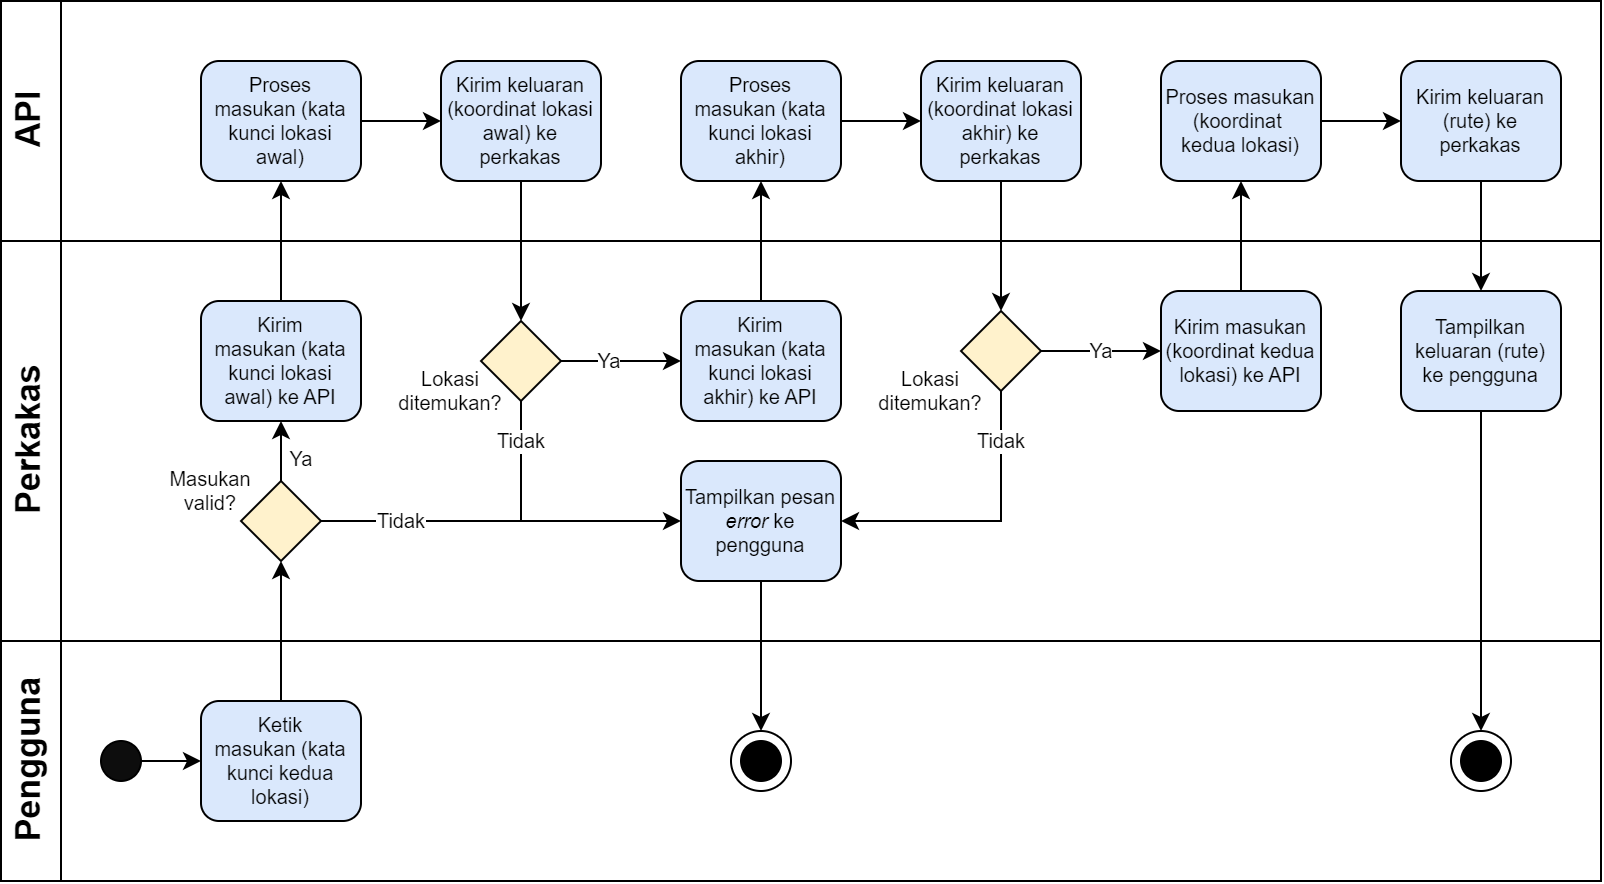
\includegraphics[width=\linewidth]{diagrams-activity-directroute}
    \caption[\textit{Activity diagram} fitur pencarian rute angkot menggunakan kata kunci lokasi]{\textit{Activity diagram} dari fitur pencarian rute angkot menggunakan kata kunci pencarian.}
    \label{fig:diagrams-activity-directroute}
\end{figure}

\begin{figure}[h]
    \centering
    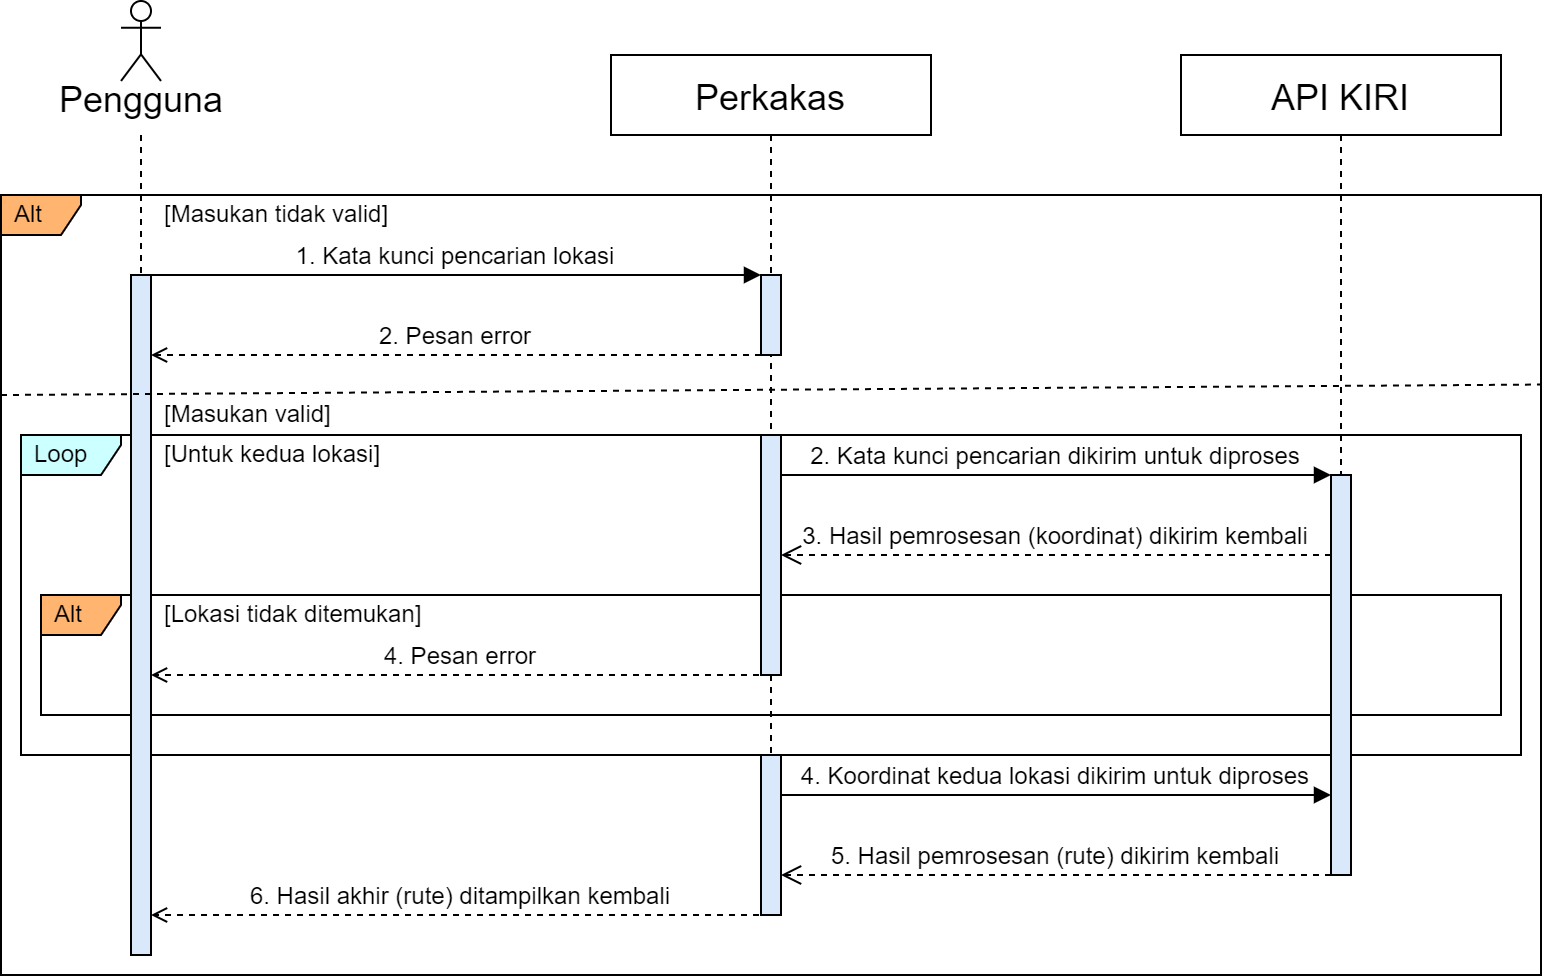
\includegraphics[width=0.8\linewidth]{diagrams-sequence-directroute}
    \caption[\textit{Sequence diagram} fitur pencarian rute angkot menggunakan kata kunci lokasi]{\textit{Sequence diagram} dari fitur pencarian rute angkot menggunakan kata kunci pencarian.}
    \label{fig:diagrams-sequence-directroute}
\end{figure}

\section{Rancangan Implementasi Perkakas}
\label{sec:design-implementation}

Bagian ini akan membahas hal-hal terkait rancangan implementasi alur kerja perkakas, seperti cara kerja perkakas, kapan dan untuk apa \textit{library-library} yang telah dibahas di Bab 2 akan digunakan, variabel-variabel utama yang diperlukan di dalam perkakas, serta hal-hal seputar fungsi-fungsi yang ada di dalam perkakas, seperti nama fungsinya, apa tujuan dari fungsi tersebut, masukan dan keluarannya, serta garis besar dari cara kerja fungsi tersebut.
\newpage\vspace*{-3.5em} % prevent widow
\subsection{Cara Kerja Perkakas}
\label{sec:design-implementation-overview}

Untuk setiap penggunaannya, perkakas \cl\xspace KIRI ini terdiri atas empat proses utama, dengan urutan operasi internal sebagai berikut.

\begin{enumerate}
	\item Penerimaan opsi dan argumen
	\begin{itemize}
		\item Perkakas akan menggunakan fungsi \verb|getopt_long| untuk menerima opsi-opsi serta argumen-argumennya dari masukan pengguna.
		\item Pemeriksaan dasar akan dilakukan di bagian ini. Maksud dari ``pemeriksaan dasar'' adalah perkakas akan mengecek apakah masukan pengguna sesuai harapan atau tidak, seperti pengecekan sintaks perintah, jumlah argumen yang dimasukkan, serta validitas opsi dan argumen yang dimasukkan.
		\item Kesalahan apapun selain kategori-kategori yang termasuk pengecekan dasar di atas hanya akan ditandai.
	\end{itemize}
	
	\item Verifikasi kebenaran opsi dan argumen
	\begin{itemize}
		\item Perkakas akan melakukan pengecekan lanjutan terhadap argumen-argumen yang dimasukkan pengguna.
		\item Perkakas akan berhenti dan mengeluarkan pesan \textit{error} yang sesuai apabila ada opsi atau argumen yang tidak valid.
	\end{itemize}	
	
	\item Pengiriman permintaan GET ke API serta penerimaan kembali respons
	\begin{itemize}
		\item Perkakas akan membangun URL yang diperlukan untuk permintaan GET. 
		\item Permintaan GET ini akan dilakukan dengan bantuan \textit{library} libcurl.
		\item \textit{Library} libcurl ini juga yang akan memfasilitasi penerimaan kembali respons dari API.
	\end{itemize}	
	
	\item Verifikasi akhir respons API
	\begin{itemize}
		\item Isi dari respons API akan diperiksa di langkah ini.
		\item Respons dari API akan berupa objek JSON, dan \textit{library} cJSON akan digunakan untuk mengkonversikan respons API ke bentuk yang dapat diproses langsung oleh perkakas.
		\item Segala abnormalitas yang terdapat di dalam isi respons tersebut akan ditangani langsung oleh perkakas dalam bentuk pesan-pesan \textit{error} untuk tiap kasusnya.
		\item Jika tidak ada hal-hal yang tidak diinginkan di dalam responsnya, maka keluaran akan ditampilkan seperti biasanya oleh perkakas.
	\end{itemize}
	
\end{enumerate}

Perhatikan bahwa \textit{library} CMake tidak disebut sama sekali di cara kerja. Hal ini dikarenakan \textit{library} ini hanya dipakai untuk fungsi \textit{cross-platform} dari perkakas, dan tidak dipakai sama sekali di seluruh proses kerja utamanya sendiri.

\subsection{Tipe Data Tambahan}
\label{sec:design-implementation-customtypes}

Bagian ini akan mendetailkan sebuah tipe data tambahan yang dibuat khusus untuk pemakaian dalam perkakas ini. Tipe data buatan ini, yang merupakan salah satu dari variabel global yang ada di perkakas ini, adalah \verb|chunk|, yang merupakan sebuah \verb|struct| (struktur) yang mengandung dua variabel internal, yaitu sebagai berikut.

\begin{itemize}
	\item \verb|data| (\verb|char *|)
	\item \verb|size| (\verb|size_t|)
\end{itemize}
\noindent
Struktur ini akan digunakan untuk variabel \verb|responsedata|, yang akan diisi dengan respons dari API KIRI setelah eksekusi proses cURL. Variabel \verb|data| di struktur ini merupakan penunjuk ke \textit{array} karakter yang akan menampung data dari respons API itu sendiri, sedangkan \verb|size|, yang merupakan sebuah \textit{unsigned integer}, akan diisi dengan ukuran dari data tersebut.

\subsection{Variabel Global}
\label{sec:design-implementation-globalvars}

Perkakas ini memiliki beberapa variabel global, yang sengaja diletakkan sebagai variabel global karena variabel-variabel ini digunakan di hampir keseluruhan dari keempat proses di subbab \ref{sec:design-implementation-overview}. Adapun variabel-variabel ini adalah sebagai berikut:

\begin{itemize}
	\item \verb|responsedata| (\verb|chunk|) \\
	Variabel ini akan diisi oleh respons dari API KIRI. Seperti yang telah dipaparkan secara singkat di subbab sebelumnya, struktur ini memiliki dua variabel, yaitu \verb|data|, yang akan berisi data responsnya sendiri, dan \verb|size|, yang merupakan ukuran dari data tersebut.
	\item \verb|responseJSON| (\verb|cJSON|) \\
	Berisi hasil konversi JSON dari respons API yang dapat dibaca oleh perkakas dan utilitas-utilitas \textit{library} cJSON.
	\item \verb|url| (\verb|char[]|) \\
	Basis dari URL yang akan digunakan sebagai URL permintaan GET ke API. Awalnya variabel ini akan berisi ``\verb|https://projectkiri.id/api?version=2|''\textemdash bagian awal ini tidak akan berubah bagaimanapun permintaan GET-nya.
	\item \verb|mode| (\verb|int|) \\
	Kode operasional perkakas berupa bilangan bulat. Bilangan ini memiliki rentang dari -1 hingga 4, dengan arti dari tiap bilangan sebagai berikut.
	
	\begin{itemize}
		\item \textbf{-1}: Mode belum didefinisikan
		\item \textbf{0}: Mode tidak valid
		\item \textbf{1}: Mode bantuan (\textit{help})
		\item \textbf{2}: Mode \textit{searchplace}
		\item \textbf{3}: Mode \textit{findroute}
		\item \textbf{4}: Mode \textit{direct}
	\end{itemize}
	
	\item \verb|region| (\verb|int|) \\
	Kode region berupa bilangan bulat untuk mode \verb|searchplace|. Bilangan ini memiliki rentang dari -1 hingga 4, di mana arti dari tiap bilangan dapat dilihat di daftar berikut.
	
	\begin{itemize}
		\item \textbf{-1}: Region belum didefinisikan
		\item \textbf{0}: Region tidak valid
		\item \textbf{1}: cgk (Cengkareng/Jakarta)
		\item \textbf{2}: bdo (Bandoeng/Bandung)
		\item \textbf{3}: mlg (Malang)
		\item \textbf{4}: sub (Surabaya)
	\end{itemize}
	
	\item \verb|query| (\verb|char[]|) \\
	\textit{String} (berupa \textit{array} karakter) yang menyimpan kata kunci pencarian lokasi untuk mode \verb|searchplace|.
	\item \verb|start| (\verb|char[]|) \\
	\textit{String} (berupa \textit{array} karakter) yang menyimpan koordinat lokasi awal (\verb|findroute|) atau kata kunci pencarian lokasi awal (\verb|direct|).
	\item \verb|finish| (\verb|char[]|) \\
	\textit{String} (berupa \textit{array} karakter) yang menyimpan koordinat lokasi akhir (\verb|findroute|) atau kata kunci pencarian lokasi akhir (\verb|direct|).
	\newpage % prevent orphan description
	\item \verb|escape| (\verb|char[]|) \\
	Variabel ini dibutuhkan karena pengkodean URL (untuk permintaan GET) tidak mendukung karakter spasi (` '), melainkan ``\verb|%20|''. \textit{String} yang karakter spasinya sudah diganti dengan ``\verb|%20|'' akan disimpan sementara di variabel ini, sebelum isinya disalin kembali ke variabel awalnya.
	\item \verb|regstart| (\verb|int|) \\
	Kode region lokasi awal berupa bilangan bulat untuk mode \verb|direct|. Bilangan ini memiliki rentang dari -1 hingga 4, dengan tiap bilangan bulat merepresentasikan region yang sama dengan kode bilangan untuk variabel \verb|region|.
	\item \verb|regfinish| (\verb|int|) \\
	Kode region lokasi akhir berupa bilangan bulat untuk mode \verb|direct|. Bilangan ini memiliki rentang dari -1 hingga 4, dengan tiap bilangan bulat merepresentasikan region yang sama dengan kode bilangan untuk variabel \verb|region|.
	\item \verb|locale| (\verb|int|) \\
	Kode bahasa berupa bilangan bulat. Bilangan ini memiliki rentang dari 0 hingga 2, dengan tiap-tiap bilangan merepresentasikan arti berikut.
	
	\begin{itemize}
		\item \textbf{0}: id (Indonesia)
		\item \textbf{1}: en (Inggris)
		\item \textbf{2}: Kode bahasa tidak valid
	\end{itemize}
	
	 Variabel ini juga merupakan satu-satunya variabel kode \textit{integer} yang, jika tidak diubah nilai awalnya (\textbf{0}), tidak akan menyebabkan \textit{error}.
	\item \verb|step| (\verb|int|) \\
	Kode khusus untuk mode \verb|direct| yang menandakan proses mana yang sedang \linebreak berlangsung\textemdash pencarian lokasi awal, pencarian lokasi akhir, atau pencarian rute.
	\item \verb|error| (\verb|int|) \\
	Kode yang menandakan apakah sebuah \textit{error} telah terjadi. Nilai awal dari variabel ini adalah \textbf{0}, dan jika variabel ini diganti menjadi \textbf{1}, di pengecekan kode \textit{error} selanjutnya, perkakas akan dihentikan.
\end{itemize}
\newpage\vspace*{-3.5em} % prevent awkward cutoff
\subsection{\texttt{print\textunderscore help()}}
\label{sec:design-code-printhelp}

Fungsi ini merupakan fungsi yang akan dipanggil ketika pengguna memilih opsi standar \verb|--help|. Keterangan singkat dari fungsi ini dapat dilihat di Tabel \ref{tab:design-code-printhelp-details}.
\vspace*{-0.25em} % prevent awkward cutoff
\begin{table}[H]
    \centering
    \caption{Detail dari fungsi \texttt{print\char`_help()}.}
    \begin{tabular}{| l | c p{10cm} |}
	\hline
		\textbf{Nama fungsi} & \multicolumn{2}{p{10.5cm} |}{\texttt{print\char`_help()}} \\
	\hline
		\textbf{Tujuan} & \multicolumn{2}{p{10.5cm} |}{Menampilkan bantuan penggunaan perkakas.} \\
	\hline
		\textbf{\textit{Input}} & \multicolumn{2}{p{10.5cm} |}{Fungsi ini tidak memerlukan masukan apapun.} \\
	\hline
		\textbf{\textit{Output}} & \multicolumn{2}{p{10.5cm} |}{Sekumpulan \textit{string} berupa bantuan penggunaan perkakas.} \\
	\hline
		\textbf{Deskripsi} & \multicolumn{2}{p{10.5cm} |}{Fungsi ini akan menampilkan bantuan penggunaan perkakas ke pengguna melalui \textit{output stream} standar (\texttt{stdout})} \\
	\hline
	\end{tabular}
    \label{tab:design-code-printhelp-details}
\end{table}
\vspace*{-1.5em} % prevent awkward cutoff
\subsection{\texttt{replace\textunderscore space()}}
\label{sec:design-code-replacespace}

Fungsi ini merupakan fungsi yang berguna untuk mengganti semua karakter spasi (` ') dalam variabel-variabel kata kunci pencarian sebelum isi dari variabel-variabel tersebut dimasukkan ke dalam URL untuk permintaan GET. Hal ini perlu dilakukan karena pengkodean HTML yang digunakan untuk format URL tidak mendukung karakter spasi, dan melainkan mensubstitusi seluruh kejadian karakter tersebut dalam suatu URL menjadi ``\%20''. Fungsi ini akan menerima sebuah \textit{array} karakter berisi URL permintaan sebagai masukannya, mengganti semua karakter spasi yang ada di dalamnya menjadi ``\%20'', dan meletakkan hasilnya di variabel global \verb|escape|. Adapun \textit{pseudocode} dari fungsi ini dapat dilihat di Algoritma \ref{alg:design-replacespace}.

\begin{algorithm}[h]
	\caption{\textendash\xspace Algoritma fungsi \texttt{replace\char`_space()}}
	\label{alg:design-replacespace}
	% input & output
	\vspace{-0.6\baselineskip}
	\begin{flushleft}
        \textbf{Input:} Sebuah \textit{string} berupa \textit{array} karakter. \\
        \textbf{Output:} \textit{String} tersebut, yang sudah diganti semua karakter spasinya ke ``\%20''. \\
	\end{flushleft}
	\vspace{-1.05\baselineskip}
	\begin{algorithmic}
		\State $j \gets 0$
		\For{$i \gets 0$ \textbf{to} size of $string$} \Comment{\textit{Loop} sampai $i$ mencapai karakter terakhir \textit{array}}
			\If{$string[i]$ == \textquotesingle\textbackslash 0\textquotesingle} \Comment{Berhenti jika $i$ sudah mencapai karakter terakhir $string$}
			    \State break 
			\EndIf
		
			\If{$string[i]$ == \textquotesingle\xspace\textquotesingle}
			    \State $escape[j] \gets$ \textquotesingle\%\textquotesingle
			    \State $escape[j + 1] \gets$ \textquotesingle 2\textquotesingle
			    \State $escape[j + 2] \gets$ \textquotesingle 0\textquotesingle
			    \State $j \gets j + 2$ \Comment{Majukan indeks $escape$ sebanyak 3 (2 + 1 di akhir fungsi)}
			\Else
				\State $escape[j] \gets string[i]$ 
			\EndIf
			\State $j \gets j + 1$
		\EndFor
		
		\State \Return{$escape$}
	\end{algorithmic}
\end{algorithm}
\vspace*{-1em} % prevent awkward cutoff
\subsection{\texttt{build\textunderscore url\textunderscore searchplace()}}
\label{sec:design-code-buildurl-searchplace}

Fungsi ini merupakan fungsi yang digunakan untuk pembangunan URL permintaan	GET untuk proses pencarian lokasi. Cara kerja fungsi ini dapat dilihat di Algoritma \ref{alg:design-buildurl-searchplace}.
	
	Selain itu, fitur ini juga memiliki implementasi tambahan yang tidak ada di API KIRI, yaitu implementasi variabel \verb|locale| untuk fitur pencarian lokasi, yang memungkinkan pemilihan bahasa Indonesia (\verb|id|) atau Inggris (\verb|en|) untuk keluaran serta pesan-pesan \textit{error} yang berhubungan dengan proses tersebut.

\begin{algorithm}[h]
	\caption{\textendash\xspace Algoritma fungsi \texttt{build\char`_url\char`_searchplace()}}
	\label{alg:design-buildurl-searchplace}
	% input & output
	\vspace{-0.6\baselineskip}
	\begin{flushleft}
        \textbf{Input:} \\
        \hspace{1.1em}\textendash\xspace $locale$: Kode bahasa \\
        \hspace{1.1em}\textendash\xspace $region$: Region dari lokasi yang ingin dicari \\
        \hspace{1.1em}\textendash\xspace $query$: Kata kunci pencarian lokasi \\
        \hspace{1.1em}\textendash\xspace $error$: Variabel penanda terjadinya \textit{error} \\
        \textbf{Output:} $url$ permintaan GET API untuk fitur pencarian lokasi \\
	\end{flushleft}
	\vspace{-1.05\baselineskip}
	\begin{algorithmic}
		\If{$locale$ == 2}
		    \State $error \gets 1$
			\State \textit{print} pesan \textit{error}: $locale$ tidak valid
			\State hentikan perkakas
		\EndIf
		
		\Switch{$region$}
			\Case{$-1$}
				\State $error \gets 1$
				\State \textit{print} pesan \textit{error} sesuai $locale$: $region$ tidak dimasukkan
				\State hentikan perkakas
			\EndCase
			\Case{$1$}
				\State tambahkan parameter $region$ \textquotesingle\textquotesingle cgk\textquotesingle\textquotesingle\xspace ke $url$
				\State break
			\EndCase
			\Case{$2$}
				\State tambahkan parameter $region$ \textquotesingle\textquotesingle bdo\textquotesingle\textquotesingle\xspace ke $url$
				\State break
			\EndCase
			\Case{$3$}
				\State tambahkan parameter $region$ \textquotesingle\textquotesingle mlg\textquotesingle\textquotesingle\xspace ke $url$
				\State break
			\EndCase
			\Case{$4$}
				\State tambahkan parameter $region$ \textquotesingle\textquotesingle sub\textquotesingle\textquotesingle\xspace ke $url$
				\State break
			\EndCase
			\Default
				\State $error \gets 1$
				\State \textit{print} pesan \textit{error} sesuai $locale$: $region$ tidak valid
				\State hentikan perkakas
			\EndDefault
		\EndSwitch
		
		\If{$query$ == \textquotesingle\textbackslash 0\textquotesingle}
		    \State $error \gets 1$
			\State \textit{print} pesan \textit{error} sesuai $locale$: $query$ tidak dimasukkan
			\State hentikan perkakas
		\Else
			\State tambahkan parameter $query$ ke $url$
		\EndIf
		
		\State tambahkan parameter kunci API ke $url$
		
		\State \Return{$url$}
	\end{algorithmic}
\end{algorithm}

\subsection{\texttt{build\textunderscore url\textunderscore findroute()}}
\label{sec:design-code-buildurl-findroute}

Fungsi ini merupakan fungsi yang digunakan untuk pembangunan URL permintaan	GET untuk proses pencarian rute angkot. Adapun alur kerja dari fungsi ini dapat dilihat di Algoritma \ref{alg:design-buildurl-findroute}.

\begin{algorithm}[h]
	\caption{\textendash\xspace Algoritma fungsi \texttt{build\char`_url\char`_findroute()}}
	\label{alg:design-buildurl-findroute}
	% input & output
	\vspace{-0.6\baselineskip}
	\begin{flushleft}
        \textbf{Input:} \\
        \hspace{1.1em}\textendash\xspace $locale$: Kode bahasa keluaran perkakas \\
        \hspace{1.1em}\textendash\xspace $start$: Koordinat \latlon\xspace lokasi awal \\
        \hspace{1.1em}\textendash\xspace $finish$: Koordinat \latlon\xspace lokasi akhir \\
        \hspace{1.1em}\textendash\xspace $error$: Variabel penanda terjadinya \textit{error} \\
        \textbf{Output:} $url$ permintaan GET API untuk fitur pencarian rute \\
	\end{flushleft}
	\vspace{-1.05\baselineskip}
	\begin{algorithmic}
	
		\Switch{$region$}
			\Case{$1$}
			    \State tambahkan parameter $locale$ \textquotesingle\textquotesingle en\textquotesingle\textquotesingle\xspace ke $url$
				\State break
			\EndCase
			\Case{$2$}
			    \State $error \gets 1$
				\State \textit{print} pesan \textit{error}: $locale$ tidak valid
				\State hentikan perkakas
			\EndCase
			\Default
				\State tambahkan parameter $locale$ \textquotesingle\textquotesingle id\textquotesingle\textquotesingle\xspace ke $url$
				\State break
			\EndDefault
		\EndSwitch
		
		\If{$start$ == \textquotesingle\textbackslash 0\textquotesingle}
		    \State $error \gets 1$
			\State \textit{print} pesan \textit{error} sesuai $locale$: $start$ tidak dimasukkan
			\State hentikan perkakas
		\Else
			\State tambahkan parameter $start$ ke $url$
		\EndIf
		
		\If{$finish$ == \textquotesingle\textbackslash 0\textquotesingle}
		    \State $error \gets 1$
			\State \textit{print} pesan \textit{error} sesuai $locale$: $finish$ tidak dimasukkan
			\State hentikan perkakas
		\Else
			\State tambahkan parameter $query$ ke $url$
		\EndIf
		
		\State tambahkan parameter presentation \textquotesingle\textquotesingle desktop\textquotesingle\textquotesingle\xspace ke $url$
		\State tambahkan parameter kunci API ke $url$
		
		\State \Return{$url$}
	\end{algorithmic}
\end{algorithm}

\subsection{\texttt{reset\textunderscore url()}}
\label{sec:design-code-buildurl-reset}

Fungsi ini digunakan untuk mengembalikan isi dari variabel \verb|url| ke nilai semula, dengan cara \mbox{mengganti} isi dari variabel tersebut kembali ke nilai awalnya, yaitu ``\verb|https://projectkiri.id/|\linebreak\verb|api?version=2|''. Penjelasan singkat dari fungsi ini terdapat di Tabel \ref{tab:design-code-buildurl-reset-details}.

\begin{table}[H]
    \centering
    \caption{Detail dari fungsi \texttt{reset\char`_url()}.}
    \begin{tabular}{| l | c p{10cm} |}
	\hline
		\textbf{Nama fungsi} & \multicolumn{2}{p{10.5cm} |}{\texttt{reset\char`_url()}} \\
	\hline
		\textbf{Tujuan} & \multicolumn{2}{p{10.5cm} |}{Mengembalikan URL ke bentuk umumnya.} \\
	\hline
		\textbf{\textit{Input}} & \multicolumn{2}{p{10.5cm} |}{\texttt{url} (variabel global)} \\
	\hline
		\textbf{\textit{Output}} & \multicolumn{2}{p{10.5cm} |}{\texttt{url} yang sudah dikembalikan nilainya} \\
	\hline
		\textbf{Deskripsi} & \multicolumn{2}{p{10.5cm} |}{Fungsi ini akan mengisi kembali nilai variabel url dengan \linebreak``\texttt{https://projectkiri.id/api?version=2}''} \\
	\hline
	\end{tabular}
    \label{tab:design-code-buildurl-reset-details}
\end{table}

\subsection{\texttt{execute\textunderscore curl()}}
\label{sec:design-code-curl-execute}

Fungsi ini digunakan untuk proses pengiriman permintaan ke API, serta penerimaan respons dari API. Semua utilitas dari library cURL yang dipakai dalam perkakas ini, seperti \textit{handler} kelebihan memori data yang masuk, dan aturan variabel apa yang akan diisi dengan data respons API, akan diimplementasikan hanya di dalam fungsi ini. Alur kerja dari fungsi ini tertera di Algoritma \ref{alg:design-curl-execute}.

\begin{algorithm}[h]
	\caption{\textendash\xspace Algoritma fungsi \texttt{execute\char`_curl()}}
	\label{alg:design-curl-execute}
	% input & output
	\vspace{-0.6\baselineskip}
	\begin{flushleft}
		\textbf{Input:} \\
		\hspace{1.1em}\textendash\xspace $responsedata$: \texttt{Chunk} (kosong) yang akan diisi respons API KIRI \\
		\hspace{1.1em}\textendash\xspace $mode$: Kode operasional perkakas \\
		\hspace{1.1em}\textendash\xspace $step$: Kode khusus mode \texttt{direct} untuk menandakan proses mana yang sedang berlangsung \\
		\textbf{Output:} $responsedata$ yang sudah diisi dengan respons API \\
	\end{flushleft}
	\vspace{-1.05\baselineskip}
	\begin{algorithmic}
		\State $curl \gets$ penunjuk ke \textit{handle} cURL
		\State $curlcode \gets$ kode respons cURL
		\State kosongkan $responsedata$ \Comment{Untuk fungsi dengan banyak langkah}
		\State inisialisasi $curl$
		
		\If{$curl \neq false$} \Comment{Selama proses cURL masih berjalan}
			\State atur opsi-opsi $curl$
			\State $curlcode \gets$ jalankan proses $curl$
			\If{$curlcode$ bukan error}
				\State \textbf{panggil fungsi:} \texttt{print\char`_curl\char`_error()}
			\EndIf
		
			\Switch{$mode$}
				\Case{$2$}
				    \State \textbf{panggil fungsi:} \texttt{write\char`_searchplace()}
					\State break
				\EndCase
				\Case{$3$}
					\State\textbf{panggil fungsi:} \texttt{write\char`_findroute()}
					\State break
				\EndCase
				\Case{$4$}
					\If{$step == 0$\xspace||\xspace$step == 1$} \Comment{Pencarian lokasi awal atau akhir}
						\State \textbf{panggil fungsi:} \texttt{write\char`_searchplace\char`_noreturns()}
						\State break
					\ElsIf{$step == 2$} \Comment{Pencarian rute}
						\State\textbf{ panggil fungsi:} \texttt{write\char`_findroute()}
						\State break
					\EndIf
				\EndCase
			\EndSwitch
			
			\State lakukan \textit{cleanup handle} $curl$
		\EndIf
		
		\State lakukan \textit{global cleanup} cURL
		
		\State \Return{$responsedata$}
	\end{algorithmic}
\end{algorithm}

\subsection{\texttt{print\textunderscore curl\textunderscore error()}}
\label{sec:design-code-curl-error}

Fungsi ini merupakan fungsi sederhana yang akan mengeluarkan pesan \textit{error} apabila terjadi \textit{error} koneksi ketika perkakas ingin melakukan komunikasi dengan API KIRI. Untuk keterangan cara kerja lebih lanjut, \textit{pseudocode} untuk fungsi ini dapat dilihat di Algoritma \ref{alg:design-curl-error}.

\begin{algorithm}[h]
	\caption{\textendash\xspace Algoritma fungsi \texttt{print\char`_curl\char`_error()}}
	\label{alg:design-curl-error}
	% input & output
	\vspace{-0.6\baselineskip}
	\begin{flushleft}
		\textbf{Input:} $error$: Variabel penanda terjadinya \textit{error} \\
		\textbf{Output:} Pesan \textit{error} yang memberitahu pengguna bahwa telah terjadi \textit{error} dalam proses cURL. \\
	\end{flushleft}
	\vspace{-1.05\baselineskip}
	\begin{algorithmic}
		\If{$error == 1$}
			\State \textit{print} pesan \textit{error} sesuai $locale$: telah terjadi error cURL
		\EndIf
	\end{algorithmic}
\end{algorithm}

\subsection{\texttt{write\textunderscore memalloc()}}
\label{sec:design-code-write-memalloc}

Fungsi ini adalah fungsi tambahan untuk libcurl yang bertugas menerima data yang masuk dari API. Di fungsi ini juga diimplementasikan sebuah \textit{handler} pengalokasian memori, yang akan menghindari terjadinya \textit{error} akibat ukuran data yang diterima melebihi alokasi memori yang diperbolehkan untuk variabel yang akan diisi dengan data tersebut. Adapun penjelasan singkat dari fungsi ini dapat dilihat di Algoritma \ref{alg:design-write-memalloc}.

\begin{algorithm}[h]
	\caption{\textendash\xspace Algoritma fungsi \texttt{write\char`_memalloc()}}
	\label{alg:design-write-memalloc}
	% input & output
	\vspace{-0.6\baselineskip}
	\begin{flushleft}
		\textbf{Input:} \\
		\hspace{1.1em}\textendash\xspace $incomingdata$: Variabel sementara untuk menampung data yang diterima dari API \\
		\hspace{1.1em}\textendash\xspace $size$: Ukuran dari satu \textit{block} data \\
		\hspace{1.1em}\textendash\xspace $nmenb$: Berapa banyak \textit{block} data yang diterima \\
		\hspace{1.1em}\textendash\xspace $userdata$: Variabel akhir yang akan diisi dengan data yang diterima dari API \\
		\textbf{Output:} $realsize$: Ukuran total data yang diterima \\
	\end{flushleft}
	\vspace{-1.05\baselineskip}
	\begin{algorithmic}
		\State $realsize \gets size * nmemb$ \Comment{Hitung ukuran data yang diterima} 
		\State $memory \gets userdata$ \Comment{Masukkan data yang diterima ke variabel tujuan}
		\State $ptr \gets$ realokasi ukuran memori dari data dalam $memory$
		
		\If{$ptr ==$ NULL} \Comment{Kalau realokasi gagal...}
			\State \textit{print} pesan \textit{error}: Memori habis
			\State \textbf{return} $0$ \Comment{Menandakan bahwa realokasi memori gagal}
		\EndIf
		
		\State Isi data dalam $ptr$ ke \textit{chunk} $memory$
		\State Perbarui ukuran data dalam \textit{chunk} $memory$
		
		\State \textbf{return} $realsize$ \Comment{Untuk verifikasi keutuhan data asli}
	\end{algorithmic}
\end{algorithm}

\subsection{\texttt{write\textunderscore searchplace()}}
\label{sec:design-code-write-searchplace}

Fungsi ini adalah fungsi yang bertugas untuk memproses respons dari API untuk fitur pencarian lokasi dari mode \verb|searchplace|. \textit{Pseudocode} dari fungsi ini tertulis di Algoritma \ref{alg:design-write-searchplace}.

\begin{algorithm}[h]
	\caption{\textendash\xspace Algoritma fungsi \texttt{write\char`_searchplace()}}
	\label{alg:design-write-searchplace}
	% input & output
	\vspace{-0.6\baselineskip}
	\begin{flushleft}
		\textbf{Input:} \\
		\hspace{1.1em}\textendash\xspace $responsedata$: \texttt{Chunk} yang sudah diisi dengan respons API KIRI \\
		\hspace{1.1em}\textendash\xspace $responseJSON$: $responsedata$ yang sudah diubah ke bentuk yang dapat diolah bahasa C \\
		\hspace{1.1em}\textendash\xspace $error$: Variabel penanda terjadinya \textit{error} \\
		\hspace{1.1em}\textendash\xspace $locale$: Kode bahasa keluaran perkakas \\
		\textbf{Output:} Keluaran akhir fitur pencarian lokasi \\
	\end{flushleft}
	\vspace{-1.05\baselineskip}
	\begin{algorithmic}
		\State $responseJSON \gets$ data dalam $responsedata$ yang diubah dari bentuk JSON
		\State $status \gets$ \textquotesingle\textquotesingle status\textquotesingle\textquotesingle\xspace dalam $responseJSON$
		
		\If{$status \neq$ \textquotesingle\textquotesingle ok\textquotesingle\textquotesingle}
			\State $error \gets 1$
			\State \textit{print} pesan \textit{error} sesuai $locale$: hasil API \textit{error}
		\Else
			\State $result \gets$ \textquotesingle\textquotesingle searchresult\textquotesingle\textquotesingle\xspace dalam $responseJSON$
			
			\If{size of $result ==$ 0}
				\State $error \gets 1$
				\State \textit{print} pesan \textit{output} sesuai $locale$: Tidak ada lokasi yang ditemukan
			\Else
				\State $indexitem \gets 1$
				
				\ForEach{$resultitem$ \textbf{in} $result$} \Comment{Untuk setiap lokasi dalam $reesult$...}
					\State $resultitemname \gets$ \textquotesingle\textquotesingle placename\textquotesingle\textquotesingle\xspace dalam $resultitem$
					\State $resultitemlocation \gets$ \textquotesingle\textquotesingle location\textquotesingle\textquotesingle\xspace dalam $resultitem$
					\State \textit{print} $resultitemname$ dan $resultitemlocation$
					\State $indexitem \gets indexitem + 1$
				\EndFor
			\EndIf
		\EndIf
	\end{algorithmic}
\end{algorithm}
	
\subsection{\texttt{write\textunderscore findroute()}}
\label{sec:design-code-write-findroute}

Fungsi ini adalah fungsi yang bertugas untuk memproses respons dari API untuk fitur pencarian rute angkot. Perlu diperhatikan bahwa ada sebuah \textit{bug} dari API KIRI di mana durasi rute dalam menit tidak diterjemahkan dari bahasa Inggris, apabila variabel \verb|locale| diatur ke bahasa Indonesia. Potongan kode untuk mengatasi \textit{bug} ini juga akan terdapat di dalam fungsi ini. Adapun penjelasan lebih lanjut dari fungsi ini dapat dilihat di Algoritma \ref{alg:design-write-findroute}.

\begin{algorithm}[h]
	\caption{\textendash\xspace Algoritma fungsi \texttt{write\char`_findroute()}}
	\label{alg:design-write-findroute}
	% input & output
	\vspace{-0.6\baselineskip}
	\begin{flushleft}
		\textbf{Input:} \\
		\hspace{1.1em}\textendash\xspace $responsedata$: \texttt{Chunk} yang sudah diisi dengan respons API KIRI \\
		\hspace{1.1em}\textendash\xspace $responseJSON$: $responsedata$ yang sudah diubah ke bentuk yang dapat diolah bahasa C \\
		\hspace{1.1em}\textendash\xspace $error$: Variabel penanda terjadinya \textit{error} \\
		\hspace{1.1em}\textendash\xspace $locale$: Kode bahasa keluaran perkakas \\
		\textbf{Output:} Keluaran akhir fitur pencarian rute \\
	\end{flushleft}
	\vspace{-1.05\baselineskip}
	\begin{algorithmic}
		\State $responseJSON \gets$ data dalam $responsedata$
		\State $status \gets$ \textquotesingle\textquotesingle status\textquotesingle\textquotesingle\xspace dalam $responseJSON$
		
		\If{$status \neq$ \textquotesingle\textquotesingle ok\textquotesingle\textquotesingle}
			\State $error \gets 1$
			\State \textit{print} pesan \textit{error} sesuai $locale$: hasil API \textit{error}
		\Else
			\State $result \gets$ \textquotesingle\textquotesingle routingresults\textquotesingle\textquotesingle\xspace dalam $responseJSON$
			\State $indexroute \gets 1$
			
			\ForEach{$route$ \textbf{in} $result$} \Comment{Untuk setiap rute dalam $reesult$...}
				\State $routesteps \gets$ \textquotesingle\textquotesingle steps\textquotesingle\textquotesingle\xspace dalam $resultitem$
				\State $routetime \gets$ \textquotesingle\textquotesingle traveltime\textquotesingle\textquotesingle\xspace dalam $resultitem$
				
				\If{$routetime ==$ NULL}
					\State $error \gets 1$
					\State \textit{print} pesan \textit{output} sesuai $locale$: Tidak ada rute yang ditemukan
				\Else
					\State $indexstep \gets 1$
					\If{$locale \neq 1$} \Comment{Betulkan bug durasi menit dalam $locale$ id}
						\State $routetimestring \gets$ hasil terjemahan ``minute'' dalam $routetime$ ke ``menit''
					\Else
						\State $routetimestring \gets routetime$
					\EndIf
					\State \textit{print} $routetimestring$
					
					\ForEach{$routestepitem$ \textbf{in} $routesteps$} \Comment{Untuk setiap langkah rute...}
						\State $routestepdetail \gets routestepitem[3]$ \\ \Comment{Langkah dalam bahasa natural ada di indeks ke-3}
						\State \textit{print $routestepdetail$}
					\EndFor
				\EndIf
				\State $indexroute \gets indexroute + 1$
			\EndFor
		\EndIf
	\end{algorithmic}
\end{algorithm}

\subsection{\texttt{write\textunderscore searchplace\textunderscore noreturns()}}
\label{sec:design-code-write-searchplacenoreturns}

Fungsi ini adalah fungsi yang bertugas untuk memproses respons dari API untuk fitur pencarian lokasi dari mode \verb|direct|. Berbeda dengan fungsi \verb|searchplace| sebelumnya, fungsi ini akan mengambil data dari variabel \verb|responsedata|, tetapi hanya akan menampilkan nama lokasi pertama yang ditemukan, atau jika terjadi \textit{error} di salah satu prosesnya, maka fitur ini akan menampilkan pesan \textit{error} yang sesuai. Adapun penjelasan lebih lanjut dari alur kerja fungsi ini dapat dilihat di Algoritma \ref{alg:design-write-searchplacenoreturns}.

\begin{algorithm}[h]
	\caption{\textendash\xspace Algoritma fungsi \texttt{write\char`_searchplace\char`_noreturns()}}
	\label{alg:design-write-searchplacenoreturns}
	% input & output
	\vspace{-0.6\baselineskip}
	\begin{flushleft}
		\textbf{Input:} \\
		\hspace{1.1em}\textendash\xspace $responsedata$: \texttt{Chunk} yang sudah diisi dengan respons API KIRI \\
		\hspace{1.1em}\textendash\xspace $responseJSON$: $responsedata$ yang sudah diubah ke bentuk yang dapat diolah bahasa C \\
		\hspace{1.1em}\textendash\xspace $error$: Variabel penanda terjadinya \textit{error} \\
		\hspace{1.1em}\textendash\xspace $step$: Kode khusus mode \texttt{direct} untuk menandakan proses mana yang sedang berlangsung. \\
		\hspace{1.1em}\textendash\xspace $locale$: Kode bahasa keluaran perkakas \\
		\textbf{Output:} Nama lokasi pertama yang ditemukan \\
	\end{flushleft}
	\vspace{-1.05\baselineskip}
	\begin{algorithmic}
		\State $responseJSON \gets$ data dalam $responsedata$
		\State $status \gets$ \textquotesingle\textquotesingle status\textquotesingle\textquotesingle\xspace dalam $responseJSON$
		
		\If{$status \neq$ \textquotesingle\textquotesingle ok\textquotesingle\textquotesingle}
			\State $error \gets 1$
			\State \textit{print} pesan \textit{error} sesuai $locale$: hasil API \textit{error}
		\Else
			\State $result \gets$ \textquotesingle\textquotesingle searchresult\textquotesingle\textquotesingle\xspace dalam $responseJSON$
			
			\If{size of $result ==$ 0}
				\State $error \gets 1$
				\State \textit{print} pesan \textit{output} sesuai $locale$: Tidak ada lokasi yang ditemukan
			\Else
				\State $indexitem \gets 1$
				
				\State $resultitem \gets result[0]$ \\
				\Comment{Mode \texttt{direct} hanya mendukung lokasi pertama yang ditemukan}
				\State $resultitemname \gets$ \textquotesingle\textquotesingle placename\textquotesingle\textquotesingle\xspace dalam $resultitem$
				\State $resultitemlocation \gets$ \textquotesingle\textquotesingle location\textquotesingle\textquotesingle\xspace dalam $resultitem$
				
				\State \textit{print} $resultitemname$
				\If{$step == 0$}
					\State $start \gets resultitemlocation$
				\ElsIf{$step == 1$}
					\State $finish \gets resultitemlocation$
				\EndIf
			\EndIf
		\EndIf
	\end{algorithmic}
\end{algorithm}

\subsection{Fungsi utama (\texttt{main()})}
\label{sec:design-code-main}

Tentunya seluruh perangkat lunak bahasa C akan memiliki satu buah fungsi utama. Untuk perkakas ini, alur kerja dari fungsi utamanya adalah sebagai berikut.

\begin{enumerate}
	\item Perkakas menerima seluruh opsi dan argumen dari masukan.
	\item Terjemahkan setiap opsi (serta argumennya, jika ada) ke nilai variabelnya masing-masing.
	\item Kalau ada kelebihan opsi/argumen atau ada opsi/argumen yang tidak tepat/valid, \textit{return} $1$ sebagai penanda bahwa perkakas keluar dengan \textit{error}, dan keluarkan pesan \textit{error} yang sesuai.
	\item Kalau semua masukan valid, lanjutkan proses sesuai variabel-variabel yang telah diterjemahkan tadi, sampai keluaran akhir dapat ditampilkan.
\end{enumerate}
\noindent
\textit{Pseudocode} dari alur kerja fungsi utama ini dapat dilihat di Algoritma \ref{alg:design-main}.

\begin{algorithm}[h]
	\caption{\textendash\xspace Alur kerja fungsi utama perkakas}
	\label{alg:design-main}
	% input & output
	\vspace{-0.6\baselineskip}
	\begin{flushleft}
		\textbf{Input:} Semua variabel yang tertulis di subbab \ref{sec:design-implementation-globalvars} \\
		\textbf{Output:} \textit{Exit code} perkakas. \\
	\end{flushleft}
	\vspace{-1.05\baselineskip}
	\begin{algorithmic}
		\While{TRUE} \Comment{Selama $getopt$ masih berlangsung...}
			\State $funct \gets$ hasil $getopt$
			
			\Switch{$funct$}
				\Case{\textquotesingle h\textquotesingle}
					\If{$mode \neq -1$} \Comment{Kalau $mode$ belum diatur...}
						\State ganti $mode$ ke mode bantuan
					\EndIf
				\EndCase
				\Case{\textquotesingle m\textquotesingle}
					\If{$mode \neq -1$}
						\State ganti $mode$ ke mode operasional yang sesuai
					\EndIf
				\EndCase
				\Case{\textquotesingle r\textquotesingle}
					\State ganti $region$ ke region yang sesuai
				\EndCase
				\Case{\textquotesingle q\textquotesingle}
					\If{Masukan untuk $query$ tidak kosong}
						\State \textit{escape} semua karakter spasi dalam masukan
						\State $query \gets$ hasil \textit{escape}
					\EndIf
				\EndCase
				\Case{\textquotesingle s\textquotesingle}
					\If{Masukan untuk $start$ tidak kosong}
						\State \textit{escape} semua karakter spasi dalam masukan
						\State $start \gets$ hasil \textit{escape}
					\EndIf
				\EndCase
				\Case{\textquotesingle f\textquotesingle}
					\If{Masukan untuk $finish$ tidak kosong}
						\State \textit{escape} semua karakter spasi dalam masukan
						\State $finish \gets$ hasil \textit{escape}
					\EndIf
				\EndCase
				\Case{\textquotesingle S\textquotesingle}
					\State ganti $regstart$ ke region yang sesuai
				\EndCase
				\Case{\textquotesingle F\textquotesingle}
					\State ganti $regfinish$ ke region yang sesuai
				\EndCase
				\Case{\textquotesingle l\textquotesingle}
					\State ganti $locale$ ke bahasa yang sesuai
				\EndCase
				\Case{\textquotesingle :\textquotesingle}
					\State $error \gets 1$
					\State \textit{print} pesan \textit{error} sesuai $locale$: Ada opsi yang kehilangan argumen
					\State hentikan perkakas
				\EndCase
				\Case{\textquotesingle ?\textquotesingle}
					\State $error \gets 1$
					\State \textit{print} pesan \textit{error} sesuai $locale$: Ada opsi yang tidak valid
					\State hentikan perkakas
				\EndCase
			\EndSwitch
		\EndWhile
	\end{algorithmic}
	\begin{flushright}
		Lanjut di halaman berikutnya...
	\end{flushright}
	\vspace{-0.95\baselineskip}
\end{algorithm}
% Belah 2 - terlalu panjang
\begin{algorithm}[h]
	\begin{center}
		\textbf{Algoritma 10} \textendash\xspace Lanjutan dari halaman sebelumnya
	\end{center}
	\begin{algorithmic}
		\If{ada kelebihan argumen}
			\State $error \gets 1$
			\State \textit{print} pesan \textit{error} sesuai $locale$: Ada kelebihan argumen
		\Else
			\Switch{$funct$}
				\Case{-1}
					\State $error \gets 1$
					\State \textit{print} pesan \textit{error} sesuai $locale$: Tidak ada masukan ke $mode$
					\State hentikan perkakas
				\EndCase
				\Case{1}
					\State \textbf{panggil fungsi}: \texttt{print\char`_help()}
				\EndCase
				\Case{2}
					\State \textbf{panggil fungsi}: \texttt{build\char`_url\char`_searchplace($region$, $query$)}
				\EndCase
				\Case{3}
					\State \textbf{panggil fungsi}: \texttt{build\char`_url\char`_findroute($locale$, $start$, $finish$)}
				\EndCase
				\Case{4}
					\State $step \gets 0$
					\State \textbf{panggil fungsi}: \texttt{build\char`_url\char`_searchplace($regstart$, $start$)}
					\State \textbf{panggil fungsi}: \texttt{execute\char`_curl()}
					\If{$error == 1$}
						\State break
					\Else
						\State \textbf{panggil fungsi}: \texttt{reset\char`_url()}
					\EndIf
					
					\State $step \gets 1$
					\State \textbf{panggil fungsi}: \texttt{build\char`_url\char`_searchplace($regfinish$, $finish$)}
					\State \textbf{panggil fungsi}: \texttt{execute\char`_curl()}
					\If{$error == 1$}
						\State break
					\Else
						\State \textbf{panggil fungsi}: \texttt{reset\char`_url()}
					\EndIf
					
					\State $step \gets 2$
					\State \textbf{panggil fungsi}: \texttt{build\char`_url\char`_findroute($locale$, $start$, $finish$)}
					\State \textbf{panggil fungsi}: \texttt{execute\char`_curl()}
				\EndCase
				\Default
					\State $error \gets 1$
					\State \textit{print} pesan \textit{error} sesuai $locale$: $mode$ tidak valid
					\State hentikan perkakas
				\EndCase
			\EndSwitch
		\EndIf
		
		\State \Return{0}
	\end{algorithmic}
\end{algorithm}
